\section{Analiza interfejsu komunikacyjnego}

Interfejs UART jest dzisiaj dostępny w~niemal wszystkich obecnych na mikrokontrolowerowych oraz w~wielu układach typu SoC. Jego popularność wynika zarówno z~(jak sama nazwa wskazuje) uniwersalnego charakteru jak i~prostoty implementacji. UART to cyfrowe urządzenie peryferyjne umożliwiające szeregową komunikację asynchroniczną. W~większości implementacji parametry komunikacji takie jak szybkość, czy format danych mogą być konfigurowane poprzez zmianę wartości odpowiednich rejestrów sterujących. Nierzadko możliwe jest też ustawienie trybu komunikacji spośród \textit{simplex}, \textit{duples} lub ~\textit{half-duples}. Interfejsy tego typu, szczególnie w~zastosowaniach przemysłowych, są często sprzęgane z~konwerterami poziomów logicznych odpowiednich dla standardów RS-232 lub RS-485.

\begin{figure}
    \centering
    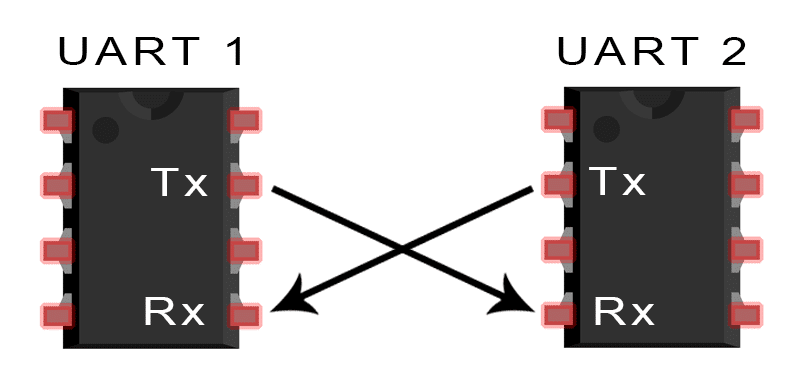
\includegraphics[scale=0.5]{img/uart.png}
    \captionsetup{format=plain,justification=centering}
    \caption{Typowa struktura komunikacji dwóch węzłów z~wykorzystaniem układu UART, źródło: \cite{uart}}
    \label{UART}
\end{figure}

Komunikacja asynchroniczna wymaga aby wszystkie węzły nadawały i~odbierały dane o~z~góry ustalonym formacie i~długości znaku (wynikającym z~szybkości transmisji). Ponadto należy wziąć pod uwagę, że zegary obecne w~poszczególnych urządzeniach mogą się z~czasem rozsynchronizowywać, a~co za tym idzie konieczny jest mechanizm ponownej synchronizacji. W~przypadku komunikacji z~wykorzystaniem modułu UART mechanizm ten wynika z~formatu przesyłanych danych. Typowa ramka składa się z~trzech elementów: \textbf{bitu startu}, \textbf{bitów danyc} oraz \textbf{bitów stopu}. Bit startu oznacza początek nowej ramki i~jest sygnalizowany stanem niskim na linii. Po nim następować może pewna liczba bitów danych - zazwyczaj $7$ lub $8$  - a~na końcu jeden lub dwa bity stopu (sygnalizowane stanem wysokim). Bit startu odpowiada za synchronizację zegarów wykorzystywanych do próbkowania stanu linii, natomiast bity stopu definiują minimalną przerwę między kolejnymi ramkami. Fakt że każdy bit startu to ponowna okazja do zsynchronizowania zegarów sprawia, że nie muszą one pracować z~dokładnie tymi samymi szybkościami. Niewielkie różnice nie powodują błędów w~odbiorze danych.

\begin{figure}
    \centering
    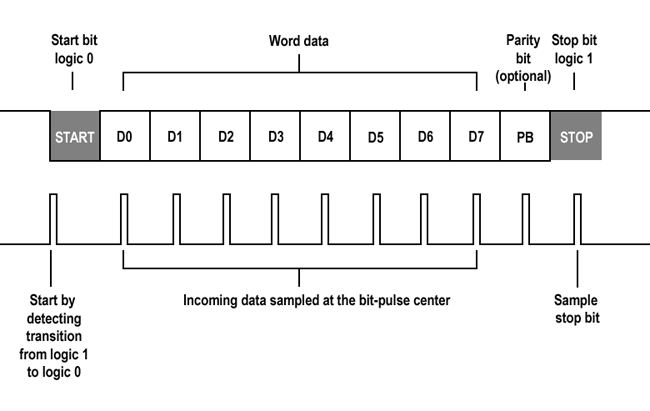
\includegraphics[scale=0.5]{img/uart_frame.png}
    \captionsetup{format=plain,justification=centering}
    \caption{Struktura ramki UART, źródło: \cite{uart_frame}}
    \label{UART}
\end{figure}

Format ramki może zostać rozszerzony o~element kontrolny w~postaci \textbf{bitu parzystości}. Jeśli występuje, przyjmuje on wartość zależną od ilości bitów w~stanie wysokim w~przesyłanych danych i~znajduje się przed bitami stopu. Możliwy jest bit parzystości (ang. \textit{even}) - ustawiony, gdy suma jest parzysta - lub nieparzystości (ang. \textit{odd}) - ustawiany, gdy suma jest nieparzysta. Dodatkowy element pozwala wykrywać ewentualne błędy transmisji. Format ramki często oznacza się w~postaci trzyznakowego identyfikatora postaci $DPS$, gdzie $D$ oznacza ilość bitów danych, $P$ - typ bitu kontrolnego ($E$ - bit parzystości, $O$ - bit nieparzystości, $N$ - brak bitu kontrolnego) a~$S$ ilość bitów stopu. Typowowymi prędkościami transmisji przez UART są:

\begin{itemize}
    \item 9600 bit/s
    \item 19200 bit/s
    \item 38400 bit/s
    \item ...
\end{itemize}

Jest to pewna zaszłość historyczna wynikająca z~częstotliwości standardowych oscylatorów dostępnych na rynku. Moduły współcześnie implementowane w~układach scalonych wzbogacone są często o~dodatkowe wyprowadzenia zegarowe umożliwiające komunikację synchroniczną. Tego typu urządzenia określane są zazwyczaj mianem USART (ang. \textit{universal synchronous asynchronous receiver-transmitter}).
